\documentclass[tikz,border=10pt]{standalone}
\usetikzlibrary{arrows.meta, positioning, calc}
\usepackage{amssymb}

\begin{document}
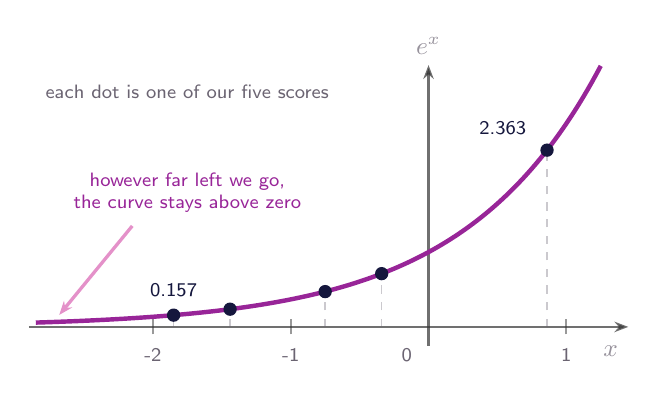
\begin{tikzpicture}[
    every node/.style={font=\sffamily},
]

\definecolor{c1}{HTML}{15173D}
\definecolor{c2}{HTML}{982598}   % the curve, and our five scores on it
\definecolor{c3}{HTML}{E491C9}
\definecolor{c4}{HTML}{F1E9E9}
\definecolor{axiscolor}{HTML}{333333}
\definecolor{labelcolor}{HTML}{6B6472}

% data coordinates, scaled by the unit vectors so the text stays put
\begin{scope}[x=1.75cm, y=0.95cm]

    % ------------------------------------------------------------ axes
    \draw[-{Stealth[length=5pt]}, line width=0.9pt, axiscolor, opacity=0.7]
        (-2.9, 0) -- (1.45, 0)
        node[anchor=north east, font=\sffamily\small, text=labelcolor,
             yshift=-3pt] {$x$};
    \draw[-{Stealth[length=5pt]}, line width=0.9pt, axiscolor, opacity=0.7]
        (0, -0.25) -- (0, 3.5)
        node[anchor=south, font=\sffamily\small, text=labelcolor] {$e^{x}$};

    \foreach \t in {-2, -1, 1} {
        \draw[axiscolor, opacity=0.5, line width=0.6pt] (\t, -0.1) -- (\t, 0.1);
        \node[font=\sffamily\scriptsize, text=labelcolor, anchor=north]
            at (\t, -0.16) {\t};
    }
    \node[font=\sffamily\scriptsize, text=labelcolor, anchor=north east]
        at (-0.05, -0.16) {0};

    % ------------------------------------------------------------ the curve
    \draw[c2, line width=1.6pt, domain=-2.85:1.25, samples=140, smooth]
        plot (\x, {exp(\x)});

    % ------------------------------------------------------------ our five scores
    \foreach \x/\y in {-1.85/0.157, -1.44/0.237, -0.75/0.472, -0.34/0.712,
                       0.86/2.363} {
        \draw[labelcolor, opacity=0.35, dashed, line width=0.5pt]
            (\x, 0) -- (\x, \y);
        \node[circle, fill=c1, inner sep=1.7pt] at (\x, \y) {};
    }

    % value labels sit next to their own dot: below the axis nothing says
    % which point they belong to. The dashed drop line gives the input, the
    % label gives the output.
    \node[font=\sffamily\scriptsize, text=c1, anchor=south]
        at (-1.85, 0.27) {0.157};
    \node[font=\sffamily\scriptsize, text=c1, anchor=south east]
        at (0.78, 2.44) {2.363};

    % ------------------------------------------------------------ the point
    \draw[c3, line width=1.2pt, -{Stealth[length=5pt]}]
        (-2.15, 1.35) -- (-2.68, 0.16);
    \node[font=\sffamily\scriptsize, text=c2, anchor=south, align=center]
        at (-1.75, 1.4) {however far left we go,\\the curve stays above zero};

    \node[font=\sffamily\scriptsize, text=labelcolor, anchor=west]
        at (-2.85, 3.15) {each dot is one of our five scores};

\end{scope}

\end{tikzpicture}
\end{document}
